\chapter{Continue reactoren en industriële processen}\label{ch:b2:continuous-reactors}

In het laboratorium voert men een reactie uit in een kolf: de reagentia gaan erin, het
mengsel wordt een uur geroerd, de reactie wordt gestopt en het product
geïsoleerd. Een fabriek die hetzelfde product per duizend ton maakt, werkt
anders. Haar reactor loopt nooit leeg: de beginstoffen stromen aan het ene uiteinde in,
de producten stromen aan het andere uit, dag en nacht, en de samenstelling binnenin
verandert niet met de tijd. Twee vragen vervangen dan ``hoe lang?'': hoe
groot moet de reactor zijn voor een gegeven \omterm{def:b2:continuous-reactors:conversion}{conversie}, en hoe wordt de warmte van
de reactie afgevoerd voordat ze de reactor onbeheersbaar opwarmt? Dit
hoofdstuk stelt de massa- en energiebalansen op voor de twee ideale
\omterm{def:b2:continuous-reactors:reactors}{continue reactoren}, de geroerde tank en de buis, vergelijkt ze, en
laat zien hoe een reactor verscheidene mogelijke toestanden kan hebben, waarvan één
op hol slaat.

\begin{recall}
Het deel van jaar~1: reactiesnelheid, snelheidswetten en ordes, geïntegreerde wetten
van een gesloten reactor (nu \omterm{def:b2:continuous-reactors:reactors}{batchreactor} genoemd), halveringstijd, de wet van
Arrhenius $k = A\,\mathrm e^{-E_a/RT}$, opeenvolgende reacties.
\Cref{ch:b2:reaction-enthalpy}: vrijgekomen warmte bij constante druk;
\cref{ch:b2:equilibrium-shifts}: \omterm{def:b2:equilibrium-shifts:single-pass}{conversie per doorgang}, \omterm{def:b2:equilibrium-shifts:single-pass}{recyclestroom}. Uit
de natuurkunde: de balans van een open systeem in stationaire stroming (wat binnenkomt min
wat buitengaat is gelijk aan wat zich ophoopt).
\end{recall}

\begin{omfigure}
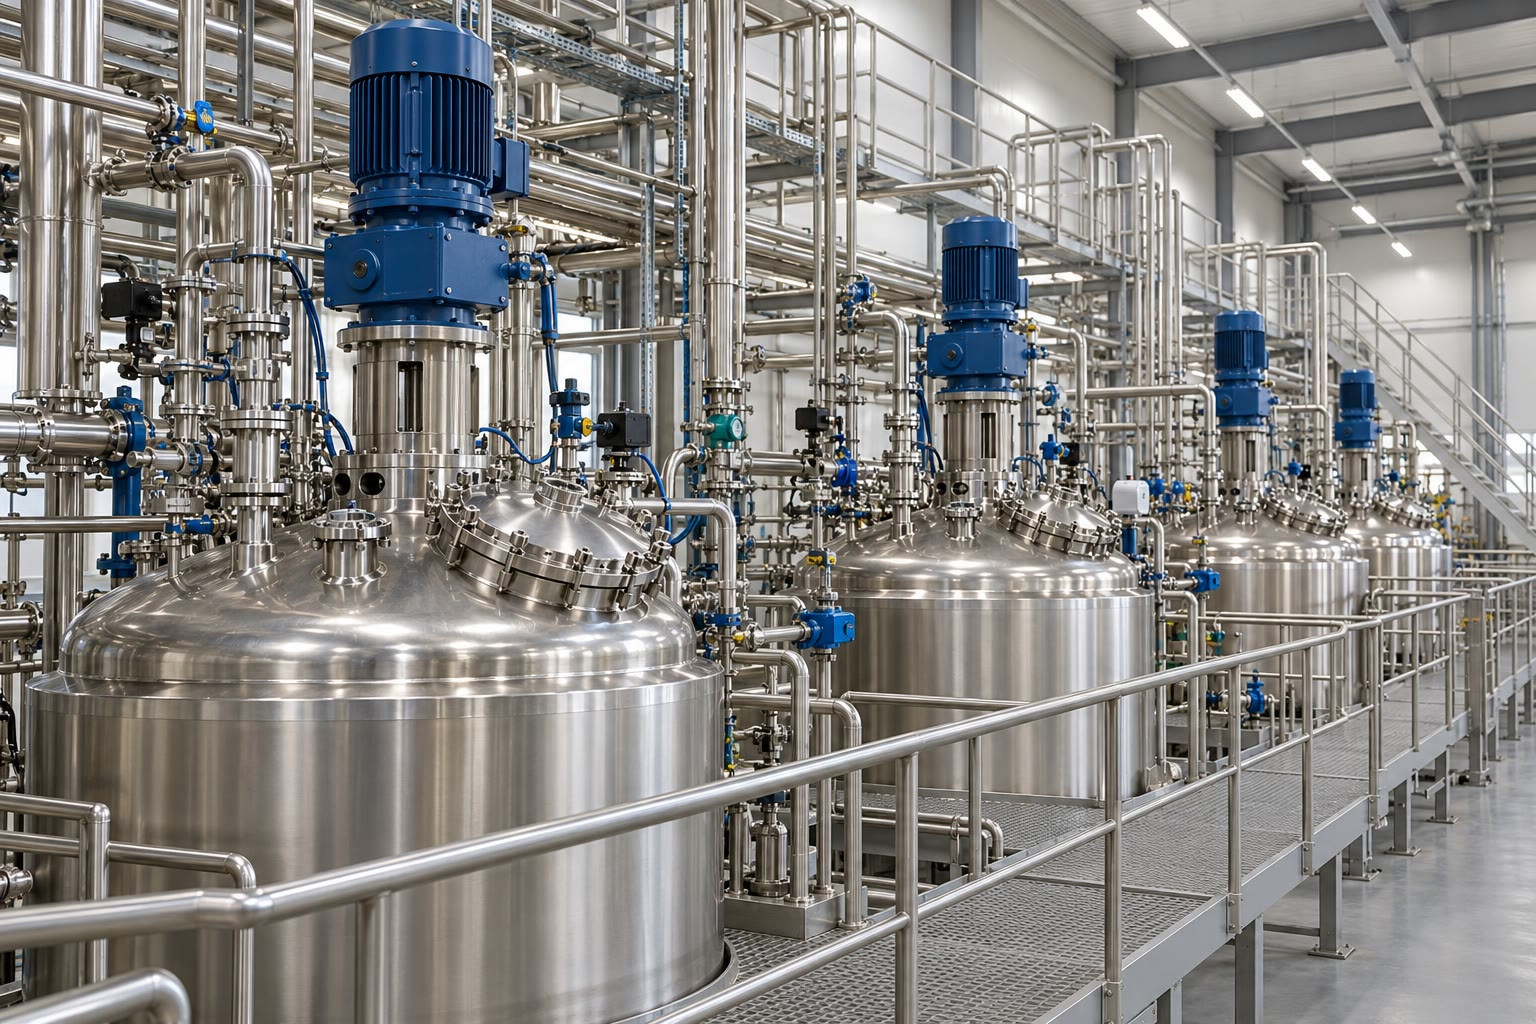
\includegraphics[width=0.6\linewidth]{images/book3/ai/b2-05-stirred-tanks.jpg}

{\small Geroerde tankreactoren in een chemische fabriek: elk vat draagt zijn
motor en tandwielkast, en de roerderas gaat omlaag in het reactiemengsel;
de leidingen brengen de voedingen aan en voeren het product en het koelwater af.}
\end{omfigure}

\section{Van batch naar continu}

\begin{definition}[Reactortypen]\label{def:b2:continuous-reactors:reactors}
Een \emph{batchreactor}\index{batchreactor} is een gesloten vat waarin de
reactie plaatsvindt zonder in- of uitstroom van materie. Een
\emph{continue reactor}\index{continue reactor} wordt doorstroomd door een stationaire
stroom van materie. Twee ideale continue reactoren dienen als model:
\begin{itemize}
  \item de \emph{continu geroerde tankreactor}\index{continu geroerde tankreactor}
(CSTR), zo goed geroerd dat de inhoud
        uniform is en dus identiek aan de stroom die hem verlaat;
  \item de \emph{propstroomreactor}\index{propstroomreactor} (PFR), een buis
        die zonder menging in de stromingsrichting door het fluïdum doorlopen wordt, waarbij elke schijf
        fluïdum als een zuiger vooruitschuift terwijl ze reageert.
\end{itemize}
\end{definition}

Een \omterm{def:b2:continuous-reactors:reactors}{continue reactor} werkt in \emph{stationaire werking} wanneer
er binnenin niets met de tijd verandert: de stromen, de temperaturen en de
samenstellingen in elk punt zijn constant. We bekijken één enkele reactie
$\mathrm A \to$ producten, met een vloeibare voeding van constante dichtheid (zodat het
volumedebiet $Q_v$ aan inlaat en uitlaat hetzelfde is), met
concentratie $c_{A,0}$ aan de inlaat.

\begin{definition}[Verblijftijd]\label{def:b2:continuous-reactors:residence-time}
De \emph{verblijftijd}\index{verblijftijd} van een \omterm{def:b2:continuous-reactors:reactors}{continue reactor} met
volume $V$, gevoed met het volumedebiet $Q_v$, is $\tau = V/Q_v$: de gemiddelde
tijd die een volume fluïdum erin doorbrengt.
\end{definition}

\begin{definition}[Conversie]\label{def:b2:continuous-reactors:conversion}
De \emph{conversie}\index{conversie} van beginstof A is $X = (F_{A,0} -
F_A)/F_{A,0}$, waarin $F_{A,0}$ en $F_A$ de molaire debieten van A zijn die de
reactor binnenkomen en verlaten; voor een \omterm{def:b2:continuous-reactors:reactors}{batchreactor} is $X = (n_{A,0} -
n_A)/n_{A,0}$. Bij constante dichtheid is $X = 1 - c_A/c_{A,0}$.
\end{definition}

De \omterm{def:b2:continuous-reactors:conversion}{conversie} slaat op één beginstof, en op een reactor of een doorgang; de
omzettingsgraad van het deel van jaar~1 slaat op een reactie en haar
beperkende beginstof. Voor één enkele reactie met A als beperkende beginstof
vallen beide samen.

\begin{proposition}[Batchreactor]\label{prop:b2:continuous-reactors:batch}
In een \omterm{def:b2:continuous-reactors:reactors}{batchreactor} met constant volume bereikt een eerste-ordereactie de
\omterm{def:b2:continuous-reactors:conversion}{conversie} $X = 1 - \mathrm e^{-kt}$ na de tijd $t$, en een tweede-ordereactie
met gelijke beginconcentraties $c_0$ de \omterm{def:b2:continuous-reactors:conversion}{conversie} $X =
kc_0t/(1 + kc_0t)$.
\end{proposition}

\begin{proof}
Dit zijn de geïntegreerde snelheidswetten van het deel van jaar~1, $c_A = c_{A,0}
\mathrm e^{-kt}$ en $1/c_A = 1/c_{A,0} + kt$, geschreven met $X = 1 -
c_A/c_{A,0}$.
\end{proof}

\section{De continu geroerde tankreactor}

\begin{omfigure}
\begin{tikzpicture}[font=\small, >={Stealth}]
  % batch
  \pic[transform shape] at (0,0) {rbflask={0.6}{omDef!20}};
  \node[below] at (0,-0.15) {batch};
  % CSTR
  \begin{scope}[xshift=4.2cm]
    \draw[thick, fill=omDef!15] (-1.2,0) rectangle (1.2,2.4);
    \draw[thick] (0,3.0) -- (0,0.5);
    \draw[thick, fill=gray!40] (-0.5,0.45) rectangle (0.5,0.6);
    \draw[thick, fill=gray!30] (-0.25,3.0) rectangle (0.25,3.35);
    \draw[->, thick, omDef] (-2.8,2.0) -- (-1.2,2.0) node[pos=0.0, above, anchor=south west, inner sep=1pt] {$Q_v$, $c_{A,0}$};
    \draw[->, thick, omThm] (1.2,0.3) -- (2.5,0.3) node[pos=1, below] {$Q_v$, $c_A$};
    \node[fill=omDef!15, inner sep=1pt] at (0.62,1.5) {$V$, $c_A$};
    \node[below] at (0,-0.15) {geroerde tank};
  \end{scope}
  % PFR
  \begin{scope}[xshift=8.4cm, yshift=1.0cm]
    \draw[thick, fill=omDef!10] (0,0) rectangle (4.2,0.7);
    \fill[omThm!25] (2.0,0) rectangle (2.35,0.7);
    \draw[thick] (2.0,0) -- (2.0,0.7) (2.35,0) -- (2.35,0.7);
    \node[above] at (2.17,0.75) {$\dd V$};
    \draw[->, thick, omDef] (-0.9,0.35) -- (0,0.35) node[pos=0, above] {$F_{A,0}$};
    \draw[->, thick, omThm] (4.2,0.35) -- (5.0,0.35) node[pos=1, above] {$F_A$};
    \node[below] at (1.0,0) {$F_A(V)$};
    \node[below] at (2.1,-1.15) {propstroombuis};
  \end{scope}
\end{tikzpicture}

{\small De drie ideale reactoren. Een batchkolf; een geroerde tank waarvan de uniforme
inhoud die van de uitlaatstroom is; een buis met propstroming, waarin
het debiet van A van schijf tot schijf afneemt.}
\end{omfigure}

\begin{proposition}[Balans van een geroerde tank]\label{prop:b2:continuous-reactors:cstr-balance}
In stationaire werking voldoet een geroerde tank met volume $V$, waarin A verdwijnt met
de snelheid $r$ (mol per liter en per seconde), aan
\[
  F_{A,0} - F_A - rV = 0, \qquad\text{dus}\qquad c_{A,0} - c_A = r\,\tau ,
\]
waarbij de snelheid geëvalueerd wordt bij de samenstelling en de temperatuur van de uitlaat.
\end{proposition}

\begin{proof}
Balans van A over de tank gedurende $\dd t$: wat binnenkomt, $F_{A,0}\dd t$,
min wat buitengaat, $F_A\dd t$, min wat reageert, $rV\dd t$, is gelijk aan de
ophoping, nul in stationaire werking. Omdat de tank uniform is, is de snelheid
overal dezelfde en gelijk aan die van de uitlaatstroom. Deel door $Q_v$.
\end{proof}

\begin{theorem}[Conversie in een geroerde tank]\label{thm:b2:continuous-reactors:cstr}
Voor een eerste-ordereactie is $X = \dfrac{k\tau}{1 + k\tau}$; voor een
tweede-ordereactie met gelijke voedingsconcentraties $c_0$ van de twee
beginstoffen is $X$ de wortel in $[0, 1]$ van $Da\,(1 - X)^2 = X$, met $Da =
kc_0\tau$.
\end{theorem}

\begin{proof}
Orde 1: $r = kc_A$, dus $c_{A,0} - c_A = k\tau c_A$, $c_A = c_{A,0}/(1 + k\tau)$
en $X = 1 - 1/(1 + k\tau)$. Orde 2: $r = kc_A^2$ (de twee concentraties blijven
gelijk), $c_0X = k\tau c_0^2(1 - X)^2$.
\end{proof}

De dimensieloze groep $Da = k\tau$ (of $kc_0\tau$), het getal van
Damköhler, vergelijkt de \omterm{def:b2:continuous-reactors:residence-time}{verblijftijd} met de tijdschaal van de reactie:
hij alleen legt de \omterm{def:b2:continuous-reactors:conversion}{conversie} vast.

\begin{method}[Een reactor dimensioneren]\label{met:b2:continuous-reactors:size-reactor}
\begin{enumerate}
  \item Schrijf de snelheidswet en de vereiste \omterm{def:b2:continuous-reactors:conversion}{conversie} $X$ op.
  \item Zoek uit de balans van de gekozen reactor het getal van Damköhler
        dat $X$ oplevert.
  \item Leid $\tau$ af uit $Da$ en de snelheidsconstante bij de werktemperatuur,
        en $V = \tau Q_v$ uit het te behandelen debiet.
\end{enumerate}
\end{method}

\section{De propstroomreactor}

\begin{theorem}[Conversie in een propstroomreactor]\label{thm:b2:continuous-reactors:pfr}
In stationaire werking volgt het debiet van A langs een propstroombuis
$\dd F_A/\dd V = -r$. Voor een eerste-ordereactie geeft dat $X = 1 -
\mathrm e^{-k\tau}$, en voor een tweede-ordereactie met gelijke voedingen $X =
Da/(1 + Da)$: de wetten van de \omterm{def:b2:continuous-reactors:reactors}{batchreactor}, met de \omterm{def:b2:continuous-reactors:residence-time}{verblijftijd} in
plaats van de tijd.
\end{theorem}

\begin{proof}
Balans van A over de schijf tussen $V$ en $V + \dd V$: $F_A(V) - F_A(V + \dd V)
- r\,\dd V = 0$, vandaar de differentiaalvergelijking. Met $F_A = Q_vc_A$ en
$\dd V = Q_v\,\dd t'$ (de tijd $t'$ die een schijf in de buis heeft doorgebracht) luidt ze
$\dd c_A/\dd t' = -r$: elke schijf is een kleine \omterm{def:b2:continuous-reactors:reactors}{batchreactor} die gedurende $\tau$ in de
buis blijft. Scheiden van de variabelen voor $r = kc_A$ geeft $c_A = c_{A,0}
\mathrm e^{-k\tau}$ aan de uitlaat; voor $r = kc_A^2$ is $1/c_A - 1/c_0 = k\tau$.
\end{proof}

\begin{omfigure}
\begin{tikzpicture}
\begin{axis}[
  width=0.75\linewidth, height=6cm, xmin=0, xmax=10, ymin=0, ymax=1.05,
  axis x line=bottom, axis y line=left, xlabel={getal van Damköhler $k\tau$},
  ylabel={conversie $X$}, tick label style={font=\small},
  label style={font=\small}, clip=false,
  legend style={font=\scriptsize, draw=none, at={(0.98,0.05)}, anchor=south east}]
\addplot[omThm, very thick] table[x=Da, y=pfr] {figdata/out/bachelor-2-reactors-a.dat};
\addplot[omProp, thick] table[x=Da, y=five] {figdata/out/bachelor-2-reactors-a.dat};
\addplot[omProp, thick, dashed] table[x=Da, y=two] {figdata/out/bachelor-2-reactors-a.dat};
\addplot[omDef, very thick] table[x=Da, y=cstr] {figdata/out/bachelor-2-reactors-a.dat};
\legend{propstroming, 5 tanks in serie, 2 tanks in serie, 1 geroerde tank}
\draw[dotted] (axis cs:2.303,0) -- (axis cs:2.303,0.9) -- (axis cs:9,0.9);
\fill[omThm] (axis cs:2.303,0.9) circle (1.4pt);
\fill[omDef] (axis cs:9,0.9) circle (1.4pt);
\end{axis}
\end{tikzpicture}

{\small \omterm{def:b2:continuous-reactors:conversion}{Conversie} van een eerste-ordereactie als functie van $k\tau$ in de ideale
reactoren. Voor 90\,\% \omterm{def:b2:continuous-reactors:conversion}{conversie} heeft een propstroombuis $k\tau = \ln 10 = 2.3$ nodig,
één geroerde tank $k\tau = 9$: viermaal het volume. Tanks in serie
benaderen de buis.}
% (model curves, computed in figdata/bachelor-2/reactors.py)
\end{omfigure}

\begin{proposition}[Tank of buis]\label{prop:b2:continuous-reactors:compare}
Voor elke snelheid die toeneemt met de concentratie van A (elke positieve
orde) bereikt een \omterm{def:b2:continuous-reactors:reactors}{propstroomreactor} een gegeven \omterm{def:b2:continuous-reactors:conversion}{conversie} met een kleiner volume
dan een geroerde tank.
\end{proposition}

\begin{proof}
Uit de balansen volgt $\tau_{\text{CSTR}} = c_{A,0}X/r(X)$ (de snelheid bij de samenstelling
aan de uitlaat) en $\tau_{\text{PFR}} = c_{A,0}\int_0^X\dd X'/r(X')$. Omdat $r$
afneemt wanneer $X$ toeneemt, is $1/r(X') \leq 1/r(X)$ op $[0, X]$, dus is de
integraal hoogstens $X/r(X)$. Grafisch, in een diagram van $1/r$ tegen $X$, is de
$\tau$ van de buis de oppervlakte onder de kromme en die van de tank de rechthoek met
hoogte $1/r(X)$ (figuur hieronder). Voor orde 1: $\ln(1 + k\tau) \leq k\tau$,
dezelfde bewering in een andere vorm.
\end{proof}

De geroerde tank werkt overal bij de uitlaatconcentratie, de laagste van
het systeem, en dus bij de laagste snelheid; de buis benut de hoge concentraties
bij haar inlaat. De voordelen van de tank liggen elders: een uniforme, gemakkelijk geregelde
temperatuur, en een eenvoudige bediening.

\begin{omfigure}
\begin{tikzpicture}
\begin{axis}[
  width=0.62\linewidth, height=5.6cm, xmin=0, xmax=1, ymin=0, ymax=22,
  axis x line=bottom, axis y line=left, xlabel={conversie $X$},
  ylabel={$1/r$ (modeleenheden)}, tick label style={font=\small},
  label style={font=\small}, clip=false]
\fill[omDef!15] (axis cs:0,0) rectangle (axis cs:0.9,10);
\addplot[omThm, fill=omThm!20, draw=none, domain=0:0.9, samples=60] {1/(1-x)} \closedcycle;
\addplot[black, very thick] table[x=X, y=invr] {figdata/out/bachelor-2-reactors-c.dat};
\draw[omDef, thick] (axis cs:0,10) -- (axis cs:0.9,10) -- (axis cs:0.9,0);
\node[omDef, font=\scriptsize, anchor=south] at (axis cs:0.45,10.2) {geroerde tank: rechthoek, $\tau = 9$};
\node[omThm, font=\scriptsize, anchor=west] (pf) at (axis cs:0.05,6.5) {propstroming: gearceerd, $\tau = \ln 10$};
\draw[omThm, ->] (axis cs:0.25,6.0) -- (axis cs:0.3,0.8);
\end{axis}
\end{tikzpicture}

{\small Levenspieldiagram van een eerste-ordereactie ($k = 1$, $c_{A,0} = 1$).
Voor 90\,\% \omterm{def:b2:continuous-reactors:conversion}{conversie} heeft de geroerde tank de hele rechthoek nodig, de propstroming
alleen de gearceerde oppervlakte onder de kromme.}
% (model, computed in figdata/bachelor-2/reactors.py)
\end{omfigure}

\begin{proposition}[Tanks in serie]\label{prop:b2:continuous-reactors:cascade}
$N$ gelijke geroerde tanks in serie, met totale \omterm{def:b2:continuous-reactors:residence-time}{verblijftijd} $\tau$, zetten een
eerste-ordereactie om tot $X_N = 1 - (1 + k\tau/N)^{-N}$, wat toeneemt met
$N$ en naar de propstroomwaarde $1 - \mathrm e^{-k\tau}$ gaat.
\end{proposition}

\begin{proof}
Elke tank deelt de concentratie door $1 + k\tau/N$. En $(1 +
k\tau/N)^{-N} = \exp[-N\ln(1 + k\tau/N)] \to \mathrm e^{-k\tau}$, want
$N\ln(1 + u/N) \to u$.
\end{proof}

\begin{definition}[Selectiviteit]\label{def:b2:continuous-reactors:selectivity}
Wanneer een beginstof verscheidene producten kan geven, is de \emph{selectiviteit}\index{selectiviteit}
voor het gewenste product B de gevormde hoeveelheid B gedeeld door de verbruikte hoeveelheid
beginstof (maal de stoichiometrische verhouding): ze zegt welk deel van
wat gereageerd heeft de goede weg is opgegaan.
\end{definition}

\begin{proposition}[Een intermediair in een tank en in een buis]\label{prop:b2:continuous-reactors:consecutive}
Voor opeenvolgende eerste-ordereacties $\mathrm A \xrightarrow{k_1} \mathrm B
\xrightarrow{k_2} \mathrm C$, met een voeding van alleen A, is de uitlaatconcentratie
van B het grootst voor $\tau = \ln(k_2/k_1)/(k_2 - k_1)$ in een
\omterm{def:b2:continuous-reactors:reactors}{propstroomreactor} en voor $\tau = 1/\sqrt{k_1k_2}$ in een geroerde tank; het
maximum is hoger in de buis.
\end{proposition}

\begin{proof}
Buis: de batchwetten van het deel van jaar~1, $c_B = c_{A,0}\frac{k_1}{k_2 - k_1}
(\mathrm e^{-k_1\tau} - \mathrm e^{-k_2\tau})$, maximaal waar de afgeleide
nul wordt, $k_1\mathrm e^{-k_1\tau} = k_2\mathrm e^{-k_2\tau}$. Tank: $c_A =
c_{A,0}/(1 + k_1\tau)$ en de balans van B, $c_B = k_1\tau c_A - k_2\tau c_B$,
geeft $c_B = c_{A,0}k_1\tau/[(1 + k_1\tau)(1 + k_2\tau)]$, waarvan de afgeleide
nul wordt wanneer $k_1k_2\tau^2 = 1$. Het vergelijken van de maxima is
\cref{exo:b2:continuous-reactors:10}.
\end{proof}

\section{Warmtebalans en veiligheid}

\begin{definition}[Adiabatische temperatuurstijging]\label{def:b2:continuous-reactors:adiabatic-rise}
De \emph{adiabatische temperatuurstijging}\index{adiabatische temperatuurstijging}
$\Delta T_{\text{ad}}$ van een reactiemengsel is de temperatuurstijging die het
zou ondergaan als de reactie volledig verliep en er geen warmte werd afgevoerd.
\end{definition}

\begin{proposition}[Adiabatische stijging van een vloeibaar mengsel]\label{prop:b2:continuous-reactors:adiabatic}
Voor een mengsel met dichtheid $\rho$ en specifieke warmtecapaciteit $c_p$, waarin
de beginstof A, bij concentratie $c_{A,0}$, reageert met de enthalpie
$\Delta_r H$ per mol A, is de temperatuurstijging bij \omterm{def:b2:continuous-reactors:conversion}{conversie} $X$ zonder
warmteverlies
\[
  \Delta T = \frac{(-\Delta_r H)\,c_{A,0}\,X}{\rho\,c_p}, \qquad
  \Delta T_{\text{ad}} = \frac{(-\Delta_r H)\,c_{A,0}}{\rho\,c_p} .
\]
\end{proposition}

\begin{proof}
Per volume-eenheid verwarmt de vrijgekomen warmte, $(-\Delta_r H)c_{A,0}X$, een
massa $\rho$ met warmtecapaciteit $c_p$ (eerste hoofdwet bij constante druk, de twee
stappen van \cref{prop:b2:reaction-enthalpy:flame}).
\end{proof}

Een verdund mengsel is veilig: een paar graden stijging. Een geconcentreerd, sterk
\omterm{def:b2:reaction-enthalpy:exothermic}{exotherm} mengsel kan zichzelf honderden kelvin opwarmen, genoeg om het
oplosmiddel te laten koken of een andere reactie te starten. En de snelheid groeit exponentieel met de
temperatuur: warmte versnelt de reactie, die daardoor sneller warmte vrijgeeft.

\begin{proposition}[Stationaire toestanden van een gekoelde geroerde tank]\label{prop:b2:continuous-reactors:steady-states}
Voor een geroerde tank met voeding bij $T_0$, gekoeld door een mantel bij $T_0$ met
warmteoverdrachtscoëfficiënt maal oppervlakte $UA$, zijn de mogelijke stationaire temperaturen
$T$ de oplossingen van
\[
  \underbrace{\Delta T_{\text{ad}}\,X(T)}_{\text{geproduceerde warmte}} =
  \underbrace{(1 + \kappa)(T - T_0)}_{\text{afgevoerde warmte}}, \qquad
  \kappa = \frac{UA}{Q_v\rho c_p},
\]
waarin $X(T) = k(T)\tau/(1 + k(T)\tau)$ voor een eerste-ordereactie. De warmteproductie is
een S-vormige kromme in $T$, de afvoer een rechte: er kunnen één of drie
snijpunten zijn.
\end{proposition}

\begin{proof}
Energiebalans van de tank in stationaire werking, per tijdseenheid: de warmte die
de reactie vrijgeeft, $(-\Delta_r H)F_{A,0}X$, vertrekt met de
uitlaatstroom, die van $T_0$ tot $T$ wordt verwarmd, $Q_v\rho c_p(T - T_0)$, en via
de mantel, $UA(T - T_0)$. Deel door $Q_v\rho c_p$. Met de wet van Arrhenius
stijgt $X(T)$ van 0 naar 1 over een smal temperatuurgebied: een S.
\end{proof}

\begin{omfigure}
\begin{tikzpicture}
\begin{axis}[
  width=0.75\linewidth, height=6.2cm, xmin=300, xmax=470, ymin=0, ymax=250,
  axis x line=bottom, axis y line=left, xlabel={tanktemperatuur $T$ (K)},
  ylabel={warmte per eenheid debiet (K)}, tick label style={font=\small},
  label style={font=\small}, clip=true]
\addplot[omThm, very thick] table[x=T, y=gen] {figdata/out/bachelor-2-reactors-b.dat};
\addplot[omDef, very thick] table[x=T, y=rem] {figdata/out/bachelor-2-reactors-b.dat};
\fill[black] (axis cs:300.03,0.04) circle (2pt);
\fill[white, draw=black] (axis cs:390.4,135.6) circle (2pt);
\fill[black] (axis cs:429.6,194.4) circle (2pt);
\node[font=\scriptsize, anchor=north west, fill=white, inner sep=1pt] at (axis cs:318,58) {koud, stabiel}; \draw[black!60] (axis cs:301.5,2) -- (axis cs:318,52);
\node[font=\scriptsize, anchor=north west] at (axis cs:393,132) {instabiel};
\node[font=\scriptsize, anchor=south east] at (axis cs:426,197) {heet, stabiel};
\node[omThm, font=\scriptsize, anchor=north west] at (axis cs:440,196) {geproduceerd};
\node[omDef, font=\scriptsize, anchor=south east] at (axis cs:452,232) {afgevoerd};
\end{axis}
\end{tikzpicture}

{\small Semenovdiagram van een gekoelde geroerde tank (modelparameters). De
geproduceerde warmte (rood) en de afgevoerde warmte (blauwe lijn) snijden elkaar driemaal. De
middelste toestand is instabiel: een beetje warmer en de productie wint, de tank
slaat op hol naar de hete toestand; een beetje koeler en hij valt terug naar de koude.}
% (model, computed in figdata/bachelor-2/reactors.py)
\end{omfigure}

De stabiliteit van elke toestand volgt uit de hellingen: in een snijpunt
waar de afvoerlijn steiler is dan de productiekromme, voert een kleine
temperatuurstijging meer warmte af dan ze produceert, en koelt de tank terug af;
waar de productiekromme steiler is, voedt een kleine stijging zichzelf. (De
rigoureuze analyse lineariseert de tijdsafhankelijke balansen; ze wordt hier
aangenomen.)

\begin{definition}[Thermische runaway]\label{def:b2:continuous-reactors:runaway}
Een \emph{thermische runaway}\index{thermische runaway} is de zichzelf versnellende
stijging van de temperatuur van een reagerend mengsel waarvan de warmteproductie,
exponentieel groeiend met de temperatuur, de warmteafvoer voorbijsteekt.
\end{definition}

\begin{method}[Warmtebalans van een reactor]\label{met:b2:continuous-reactors:heat-balance}
\begin{enumerate}
  \item Bereken de \omterm{def:b2:continuous-reactors:adiabatic-rise}{adiabatische temperatuurstijging}: als die een paar kelvin bedraagt, is de
        reactor thermisch veilig.
  \item Bereken anders het koelvermogen, $(-\Delta_r H)F_{A,0}X$ min de
        warmte die de uitlaatstroom meevoert, en controleer dat de mantel of de spiraal
        het kan afvoeren.
  \item Controleer de stabiliteit van het werkpunt (hellingen in een
        semenovdiagram), en wat er zou gebeuren als de koeling uitviel: de
        maximaal bereikte temperatuur, $T + \Delta T_{\text{ad}}(1 - X)$ voor
        de beginstof die nog aanwezig is.
\end{enumerate}
\end{method}

\section{Van protocol naar fabriek}

Een synthese die in een kolf van \qty{1}{L} werkt, laat zich niet zomaar duizendvoudig
opschalen. Het volume, en de vrijgekomen warmte, groeien met de derde macht van de
afmeting; de wand, waardoor de warmte vertrekt, met de tweede macht. Een vat dat tien
keer breder is, heeft duizendmaal het volume maar slechts honderdmaal het
koeloppervlak: een reactie die in de kolf lauw bleef, kan in de
tank op hol slaan. De industriële praktijk voegt daarom het meest reactieve reagens
langzaam toe (de reactie kan niet meer warmte vrijgeven dan het toegevoerde reagens), verdunt,
koelt met inwendige spiralen, of stapt over op \omterm{def:b2:continuous-reactors:reactors}{continue reactoren} met een klein volume,
waarvan de kleine inhoud beperkt wat er mis kan gaan.

De \omterm{def:b2:continuous-reactors:selectivity}{selectiviteit} is de andere zorg. Een fabriek gooit niet weg wat niet
gereageerd heeft: ze scheidt het product af en voert de beginstoffen terug, zoals in de
ammoniakkringloop. Ze kan daarom een bescheiden \omterm{def:b2:equilibrium-shifts:single-pass}{conversie per doorgang} aanvaarden als de
\omterm{def:b2:continuous-reactors:selectivity}{selectiviteit} hoog is, want elk bijproduct is verloren grondstof en afval dat
verwerkt moet worden.

\begin{inthelab}[Een geroerde tank op de labtafel]
De kinetiek van een reactie die bestemd is voor een continue fabriek, wordt gemeten in een
kleine geroerde reactor die door twee geijkte pompen gevoed wordt, met een geleidbaarheidscel
of een in-lijnspectrometer aan de uitlaat. Door het debiet te variëren varieert $\tau$;
de stationaire uitlaatconcentratie bij elke $\tau$ geeft rechtstreeks de snelheid, via de
balans $r = (c_{A,0} - c_A)/\tau$, zonder enige integratie.
\end{inthelab}

\section{Oefeningen}

\begin{exercise}[$\star$]\label{exo:b2:continuous-reactors:1}
Een geroerde tank van \qty{2.0}{m^3} wordt gevoed met \qty{0.50}{L/s}. Bereken zijn
\omterm{def:b2:continuous-reactors:residence-time}{verblijftijd} in seconden en in uren.
\end{exercise}

\begin{exercise}[$\star$]\label{exo:b2:continuous-reactors:2}
Een eerste-ordereactie heeft $k = \qty{1.2e-3}{s^{-1}}$ bij de
werktemperatuur. Bereken de \omterm{def:b2:continuous-reactors:conversion}{conversie} in een geroerde tank en in een propstroombuis
met dezelfde \omterm{def:b2:continuous-reactors:residence-time}{verblijftijd}, \qty{30}{min}.
\end{exercise}

\begin{exercise}[$\star$]\label{exo:b2:continuous-reactors:3}
Welke \omterm{def:b2:continuous-reactors:residence-time}{verblijftijd} in propstroming geeft 99\,\% \omterm{def:b2:continuous-reactors:conversion}{conversie} van een eerste-ordereactie
met $k = \qty{0.020}{s^{-1}}$? En in een geroerde tank?
\end{exercise}

\begin{exercise}[$\star$]\label{exo:b2:continuous-reactors:4}
Een waterige oplossing van \qty{0.50}{mol/L} van een beginstof waarvan de reactie
\qty{-120}{kJ/mol} vrijgeeft ($\rho = \qty{1.0}{kg/L}$, $c_p =
\qty{4.2}{J/(g.K)}$), reageert volledig. Bereken de \omterm{def:b2:continuous-reactors:adiabatic-rise}{adiabatische temperatuurstijging}.
Is een uitval van de koeling gevaarlijk?
\end{exercise}

\begin{exercise}[$\star\star$]\label{exo:b2:continuous-reactors:5}
Bereken voor een tweede-ordereactie met gelijke voedingen ($kc_0 = \qty{0.010}{s^{-1}}$)
de \omterm{def:b2:continuous-reactors:residence-time}{verblijftijd} voor 80\,\% \omterm{def:b2:continuous-reactors:conversion}{conversie} in een geroerde tank en in een
propstroombuis. Vergelijk de verhouding met die van een eerste-ordereactie.
\end{exercise}

\begin{exercise}[$\star\star$]\label{exo:b2:continuous-reactors:6}
Drie gelijke geroerde tanks in serie, met een totale \omterm{def:b2:continuous-reactors:residence-time}{verblijftijd} van \qty{10}{min},
verwerken een eerste-ordereactie met $k = \qty{0.50}{min^{-1}}$. Bereken de
\omterm{def:b2:continuous-reactors:conversion}{conversie} en vergelijk met één tank en met een buis met dezelfde totale
\omterm{def:b2:continuous-reactors:residence-time}{verblijftijd}.
\end{exercise}

\begin{exercise}[$\star\star$]\label{exo:b2:continuous-reactors:7}
Een geroerde tank zet 70\,\% van een beginstof om (eerste orde). Het debiet wordt
verdubbeld. Wat is de nieuwe \omterm{def:b2:continuous-reactors:conversion}{conversie}? Met welke factor moet het volume groeien om
weer 70\,\% te halen?
\end{exercise}

\begin{exercise}[$\star\star$]\label{exo:b2:continuous-reactors:8}
Een tank van \qty{5.0}{m^3} werkt bij \qty{350}{K} met een voeding van
\qty{2.0}{mol/L} beginstof bij \qty{1.0}{L/s}, voor 90\,\% omgezet, $\Delta_r H
= \qty{-80}{kJ/mol}$, $\rho c_p = \qty{4.0}{kJ/(L.K)}$, voeding bij \qty{330}{K}.
Bereken de warmte die per seconde vrijkomt, de warmte die door de uitlaatstroom
wordt meegevoerd, en het koelvermogen van de mantel.
\end{exercise}

\begin{exercise}[$\star\star$]\label{exo:b2:continuous-reactors:9}
Een kolf van \qty{1.0}{L} en een reactor van \qty{1.0}{m^3} hebben dezelfde vorm.
Met welke factor worden het volume, de wandoppervlakte en hun verhouding
vermenigvuldigd? Leg uit waarom een reactie die in de kolf gemakkelijk te koelen is, in de reactor
op hol kan slaan.
\end{exercise}

\begin{exercise}[$\star\star\star$]\label{exo:b2:continuous-reactors:10}
Bereken voor $\mathrm A \to \mathrm B \to \mathrm C$ met $k_1 = \qty{0.10}{min^{-1}}$
en $k_2 = \qty{0.050}{min^{-1}}$ de optimale \omterm{def:b2:continuous-reactors:residence-time}{verblijftijd} en het
maximale rendement aan B in een \omterm{def:b2:continuous-reactors:reactors}{propstroomreactor} en in een geroerde tank, en leg uit
waarom de buis het beter doet voor een intermediair.
\end{exercise}

\begin{exercise}[$\star\star\star$]\label{exo:b2:continuous-reactors:11}
Beschrijf met het semenovdiagram van het hoofdstuk wat er gebeurt wanneer de
temperatuur van het koelmiddel langzaam verhoogd en daarna weer langzaam verlaagd wordt: toon aan dat
de tank bij één temperatuur van de koude naar de hete tak springt en bij een
andere terug (hysterese).
\end{exercise}

\begin{exercise}[$\star\star\star$]\label{exo:b2:continuous-reactors:12}
Een \omterm{def:b2:continuous-reactors:reactors}{batchreactor} wordt gevuld met \qty{2.0}{mol/L} beginstof ($\Delta_r H =
\qty{-100}{kJ/mol}$, $\rho c_p = \qty{4.0}{kJ/(L.K)}$) en verwarmd tot de
werktemperatuur. Dan valt de koeling uit bij 25\,\% \omterm{def:b2:continuous-reactors:conversion}{conversie}. Bereken de
temperatuur die het mengsel kan bereiken. In semibatchbedrijf wordt dezelfde
beginstof langzaam toegevoegd en verbruikt naarmate ze aankomt, zodat hoogstens 5\,\%
van de lading onomgezet aanwezig is: wat is nu de stijging in het slechtste geval?
\end{exercise}

\section{Probleem: zeep in een tank}

\begin{problem}[{Weekendprobleem --- de verzeping van een ester in een
geroerde tank: kinetiek, dimensionering voor 90\,\% conversie, de alternatieven van een
buis en van een cascade, en de warmtebalans}]
\label{pb:b2:continuous-reactors:1}
Ethylethanoaat wordt verzeept door natriumhydroxide,
\ce{CH3COOC2H5 + OH- -> CH3COO- + C2H5OH}, een tweede-ordereactie (eerste
orde in elke beginstof). Een fabriek verwerkt \qty{0.50}{L/s} van een mengsel waarvan de
concentraties ester en hydroxide aan de inlaat allebei $c_0 =
\qty{0.10}{mol/L}$ zijn. Neem voor dit probleem $k = \qty{0.11}{L/(mol.s)}$ bij de
werktemperatuur en $\Delta_r H = \qty{-55}{kJ/mol}$ (waarden vastgelegd voor de
oefening); het mengsel heeft de dichtheid en de warmtecapaciteit van water,
$\rho = \qty{997}{kg/m^3}$, $c_p = \qty{4.18}{kJ/(kg.K)}$.

\medskip
\noindent\textbf{Deel I --- Kinetiek.}
\begin{enumerate}
  \item Schrijf de snelheidswet op. Waarom blijven de twee concentraties gelijk?
  \item Hoe lang duurt 90\,\% \omterm{def:b2:continuous-reactors:conversion}{conversie} in een batchkolf?
  \item Bereken de halveringstijd in de kolf. Waarom hangt die af van $c_0$?
  \item Schrijf het getal van Damköhler van de reactie op voor een \omterm{def:b2:continuous-reactors:residence-time}{verblijftijd} $\tau$.
\end{enumerate}

\medskip
\noindent\textbf{Deel II --- Eén geroerde tank.}
\begin{enumerate}[resume]
  \item Schrijf de balans van ester in de tank op in stationaire werking.
  \item Toon aan dat $Da\,(1 - X)^2 = X$.
  \item Bereken het getal van Damköhler dat nodig is voor $X = 0.90$.
  \item Bereken de \omterm{def:b2:continuous-reactors:residence-time}{verblijftijd}.
  \item Bereken het volume van de tank.
  \item Welke concentratie ``ziet'' de reactie overal in de tank,
        en waarom is de tank zo groot?
\end{enumerate}

\medskip
\noindent\textbf{Deel III --- Een buis, een cascade.}
\begin{enumerate}[resume]
  \item Bereken het getal van Damköhler en het volume van een propstroombuis voor
        dezelfde taak.
  \item Bereken de verhouding van de twee volumes.
  \item Drie gelijke tanks in serie: schrijf het verband op tussen de
        uitlaatconcentraties van twee opeenvolgende tanks.
  \item Het totale volume van de drie tanks dat 90\,\% geeft, is
        \qty{0.85}{m^3}. Controleer dat door de concentratie te berekenen die elke
        tank verlaat.
  \item Welke opstelling zou je bouwen, en waarom zou men toch nog voor één tank
        kunnen kiezen?
\end{enumerate}

\medskip
\noindent\textbf{Deel IV --- Warmte.}
\begin{enumerate}[resume]
  \item Bereken de \omterm{def:b2:continuous-reactors:adiabatic-rise}{adiabatische temperatuurstijging} van het mengsel.
  \item Bereken de warmte die per seconde in de tank vrijkomt.
  \item Is koeling nodig? Is een runaway mogelijk?
  \item Wat zou er veranderen voor een mengsel dat met \qty{2.0}{mol/L} gevoed wordt?
  \item Bereken de massa natriumethanoaat die per dag geproduceerd wordt.
  \item Als de reactie bij een hogere temperatuur wordt uitgevoerd, hoe verandert dan het
        tankvolume, en wat is de prijs?
  \item Geef het volume van de enkele geroerde tank die 90\,\% van
        de ester omzet bij deze voeding.
\end{enumerate}
\end{problem}
